% !TEX root =  ../main_manuscript.tex 
\section{Introduction}

Patients with low- and very low-risk screening-detected localized prostate cancer (PCa) are usually advised active surveillance (AS) instead of immediate radical treatment \citep{briganti2018active}. In AS, PCa progression is routinely monitored via prostate-specific antigen (PSA), digital rectal examination, and the Gleason score from repeat prostate biopsies. Among these, the Gleason score is the strongest indicator of cancer related outcomes. Thus, patients are commonly advised curative treatment upon disease reclassification \citep{bul2013active}, which is detected via upgrade in biopsy Gleason score.

Since biopsies are scheduled intermittently, disease reclassification is always detected with a delay. The smaller the delay is, the larger is the window of opportunity for curative treatment. To this end, majority of the AS programs worldwide, schedule biopsies every 12-24 months for all patients \citep{nieboer2018active,loeb2014heterogeneity}. Such fixed and frequent biopsies may benefit a small proportion of men with a high risk of reclassification. However, for many of the \textit{slow progressing} patients (see Figure \ref{fig:npmle_plot}) frequent biopsies are redundant . Biopsies are also invasive, painful and prone to medical complications. The unnecessary burden of biopsies, and patient non-compliance \citep{bokhorst2015compliance} to frequent biopsies, has raised questions about the optimal time interval between subsequent biopsies \citep{inoue2018comparative, bratt2013study}.

\begin{figure}[!htb]
\centerline{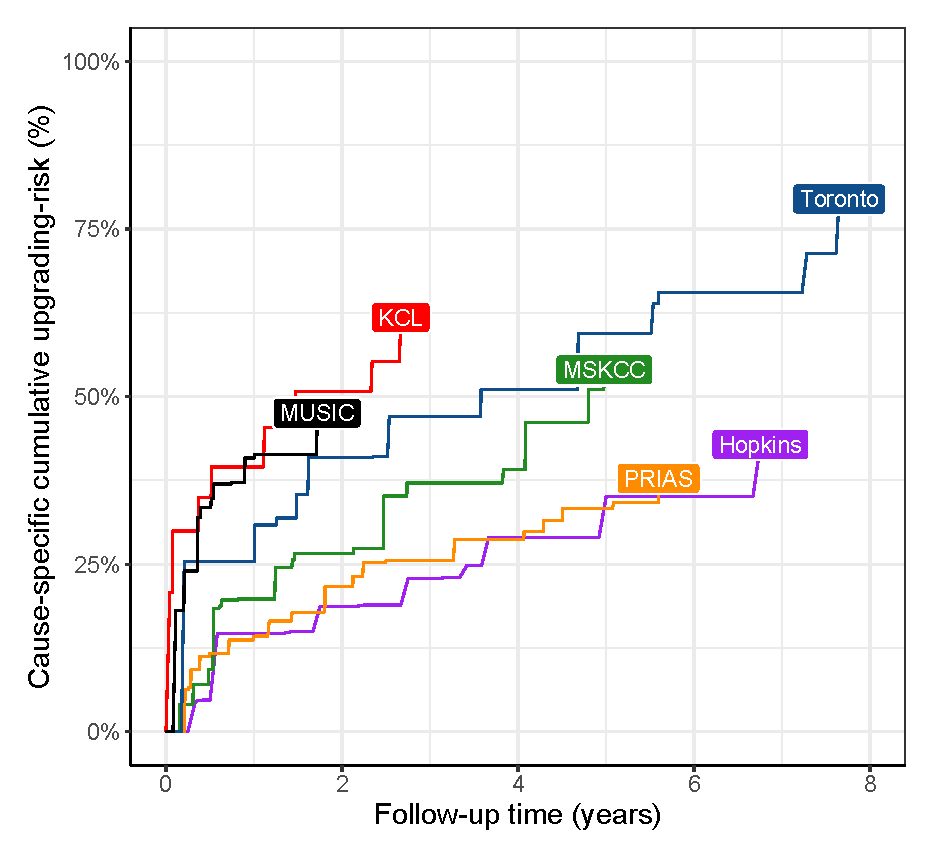
\includegraphics[width=\columnwidth]{images/npmle_plot.eps}}
\caption{\textbf{Active Surveillance Cancer Patients Are Often \textit{Slowly Progressing}}. Graph shows estimated cumulative risk of reclassification\citep{bul2013active} in AS in five of the largest AS studies that are part of the GAP3 database \citep{gap3_2018}. In all cohorts except KCL, roughly 50\% patients do not require any biopsy in first five years. In the world's largest AS cohort PRIAS and in JHAS, roughly 50\% patients do not require any biopsy in the first ten years. \textbf{Legend}: \textit{JHAS}: Johns Hopkins Active Surveillance, \textit{PRIAS}: Prostate Cancer International Active Surveillance, \textit{Toronto}: University of Toronto Active Surveillance, \textit{MSKCC}: Memorial Sloan Kettering Cancer Center Active Surveillance, \textit{KCL}: King's College London Active Surveillance}
\label{fig:npmle_plot}
\end{figure}

The simplest solution to frequent biopsies is reducing the frequency of biopsies for all patients. However, simulation studies have suggested that reducing the frequency beyond 24 months may not leave sufficient window of opportunity for curative treatment \citep{inoue2018comparative}. Although, with a gap of 24 months up to five unnecessary biopsies over ten years of follow-up may still be scheduled for the \textit{slow progressing} patients. A promising alternative to such fixed rules is biopsy decisions based on the risk of reclassification. Consider for instance the two patients shown in Figure \ref{fig:riskBasedExample}. Both patients had their latest biopsy at year one of follow-up and are now scheduled for a biopsy after a 24 month gap at year three. The PSA profile of patient A is stable and the PSA profile of patient B is rising. Since the risk of reclassification for patient A (vice-versa for patient B) is very low, he may not be subjected to unnecessary biopsy at year three.

\begin{figure}[!htb]
\centerline{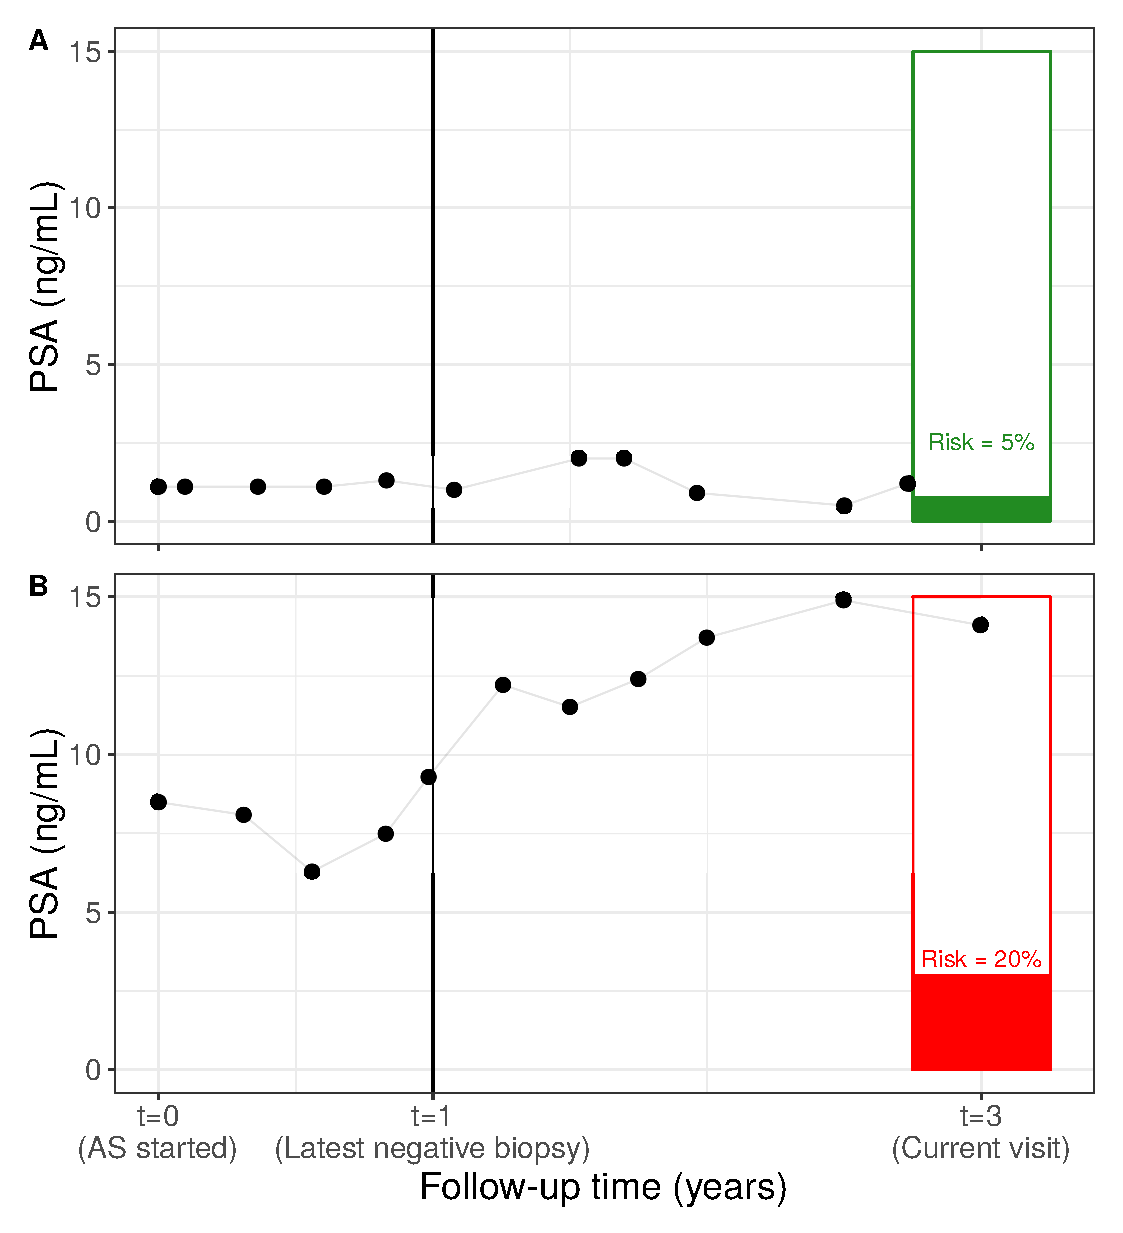
\includegraphics[width=\columnwidth]{images/riskBasedExample.eps}}
\caption{\textbf{Motivation for risk based decisions of biopsy}: Patient A and B had their latest biopsy at year one of follow-up. Patient A's prostate-specific antigen (PSA) profile remained stable until the current visit time at year three. Consequently, his cumulative risk of reclassification at year three is 5\%. On the other hand patient B's PSA profile has shown a rise since the latest biopsy, and his cumulative risk of reclassification is also 20\%. Patient B is a better candidate for biopsy than Patient A.}
\label{fig:riskBasedExample}
\end{figure}

The first challenge in the risk based approach is consolidation of observed patient data. An approach is to combine information from PSA profile with the results of previous biopsies to provide an estimate of the risk of reclassification (Figure \ref{fig:riskBasedExample}). To this end, previous studies have employed joint models for time-to-event and longitudinal data \citep{rizopoulos2012joint,tomer2019,coley2017prediction}. A subsequent challenge however, is to translate these risk estimates into decisions of biopsy (or wait). A 10\% risk can be perceived as high or low depending upon the patient's age and comorbidities. In order to make decisions patients not only require estimates of the risk, but also the estimates of consequences of a decision. Two important consequences are the delay in detection of reclassification, and the total burden of biopsies. As with the risks the consequences should also be personalized, and should be dynamically updated as more data is gathered over follow-up. Thus a complete framework for shared decision making of biopsies is required.

The goal of this work is to help patients and doctors make better decisions of biopsies than fixed and frequent biopsies. To this end, we first fit a prediction (joint) model to the world's largest AS dataset, PRIAS. Subsequently, we validate our model in multiple external cohorts that are part of the GAP3 database. Using the personalized risk predictions, we then propose the aforementioned framework for shared decision making of biopsies. Lastly, we implement the decision making framework as a web-application, and demonstrate it with real patient data.